\documentclass[11pt,a4paper]{article}
\usepackage[margin=2.3cm]{geometry}
\usepackage[T1]{fontenc}
\usepackage{lmodern}
\usepackage{amsmath}
\usepackage{graphicx}
\usepackage{booktabs}
\usepackage{caption}
\usepackage[hidelinks]{hyperref}
\graphicspath{{../figures/}}
\captionsetup{font=small}

\newcommand{\mfl}{m_{4\ell}}
\newcommand{\GeV}{\,\text{GeV}}

\title{The Higgs boson in $H\to ZZ^*\to 4\ell$ with ATLAS Open Data:\\
mass, significance and a classifier}
\author{Mohamed Ali Kabiri\\Al Akhawayn University in Ifrane, Morocco}
\date{}

\begin{document}
\maketitle

\begin{abstract}
\noindent
Using the ATLAS Open Data for education (13\,TeV, 2015--2016, 36.6\,fb$^{-1}$), I reproduce
the official four-lepton notebook exactly, correct its selection and its significance
estimate, and extend it in three ways. An unbinned likelihood fit, calibrated and validated
with 2000 toy experiments, gives $m_H = 125.06^{+0.93}_{-0.92}\GeV$ (statistical only). A
profile-likelihood fit of the $\mfl$ spectrum gives an observed significance of $3.96\sigma$
(expected $6.64\sigma$) and a signal strength $\hat\mu = 0.72^{+0.22}_{-0.20}$. A classifier
on lepton kinematics, tested on events it never saw, does not improve the expected
significance. All choices were fixed on simulation before the data were fitted, and every
number below is produced by one script, \texttt{scripts/make\_all.py}.
\end{abstract}

\section{Data, simulation and selection}

The Higgs boson was discovered in 2012 by ATLAS and CMS~\cite{atlas2012,cms2012}, with the
four-lepton channel among the most sensitive: its final state is fully reconstructed and its
background is small. This analysis uses the ATLAS Open Data release
\texttt{2025e-13tev-beta}~\cite{opendata}, skim \texttt{exactly4lep}: 1.36 million data events
and simulated samples for the signal ($m_H = 125\GeV$, eight production and decay samples),
the irreducible $ZZ^*$ background, and smaller backgrounds ($Z$+jets, $t\bar t$, $t\bar tV$,
$VVV$). Each simulated event has the weight
\begin{equation}
w = \frac{L\,\sigma\,\epsilon_\text{filter}\,k\; w_\text{MC}\; \prod SF}{\sum w_\text{MC}},
\qquad L = 36.6\,\text{fb}^{-1},
\end{equation}
with the pile-up, electron, muon and trigger scale factors $SF$. Masses and energies are in GeV.

\paragraph{Reproducing the notebook.}
The official notebook \texttt{HZZAnalysis.ipynb}~\cite{notebook} requires a trigger and a
trigger-matched lepton, $p_T > 20, 15, 10\GeV$ for the first three leptons, identification
and isolation, a lepton-flavour sum compatible with $ee\mu\mu$, $4e$ or $4\mu$, and zero total
charge. It quotes $(S+B)/\sqrt{B+0.3B^2} = 4.43$ in the window $122.5<\mfl<130\GeV$. My
implementation reproduces its stored outputs to machine precision: $S+B = 28.729$,
$B = 10.301$, metric 4.426. Three shortcuts appear on the way. The printed ``$N_\text{sig}$''
is signal plus background ($S = 18.428$). The $0.3B^2$ term corresponds to a background
uncertainty of $\sqrt{0.3} = 55\%$, not 30\%. The $p_T$ thresholds are applied to stored lepton
positions, and leptons are stored electrons first, not ordered in $p_T$. The notebook also
takes the absolute value of every weight factor.

\paragraph{Corrected selection.}
I apply the $p_T$ thresholds to $p_T$-ordered leptons, use signed weights, and pair the
leptons into $Z$ candidates: $Z_1$ is the same-flavour, opposite-charge pair closest to
$m_Z$, $Z_2$ the remaining pair, with $50 < m_{12} < 106\GeV$ and $m_{34} > 12\GeV$. The
pairing rejects charge-zero combinations such as $e^+e^+\mu^-\mu^-$, which pass the notebook's
sums; in practice no data event has that topology, and the mass cuts do the work. In the
window, the median significance of a counting experiment with known
background~\cite{cowan2011},
\begin{equation}
Z_A = \sqrt{2\left[(s+b)\ln(1+s/b) - s\right]},
\end{equation}
rises from 4.70 (notebook selection) to 4.83 with all eight signal samples, 4.91 with signed
weights, 6.42 with ordered $p_T$ cuts, and 7.82 with the $Z$ pairing ($S = 28.8$, $B = 6.6$). Figure~\ref{fig:m4l} shows the
spectrum. With signed weights, the data exceed the simulation by 40\% at $180$--$250\GeV$,
where $ZZ^*$ dominates; the weight normalization was checked against the unskimmed sample, so
the deficit is more likely a missing process (no $gg\to ZZ^*$ sample is in the list). This
deficit sets the background treatment of Section~\ref{sec:significance}.

\begin{figure}[t]
\centering
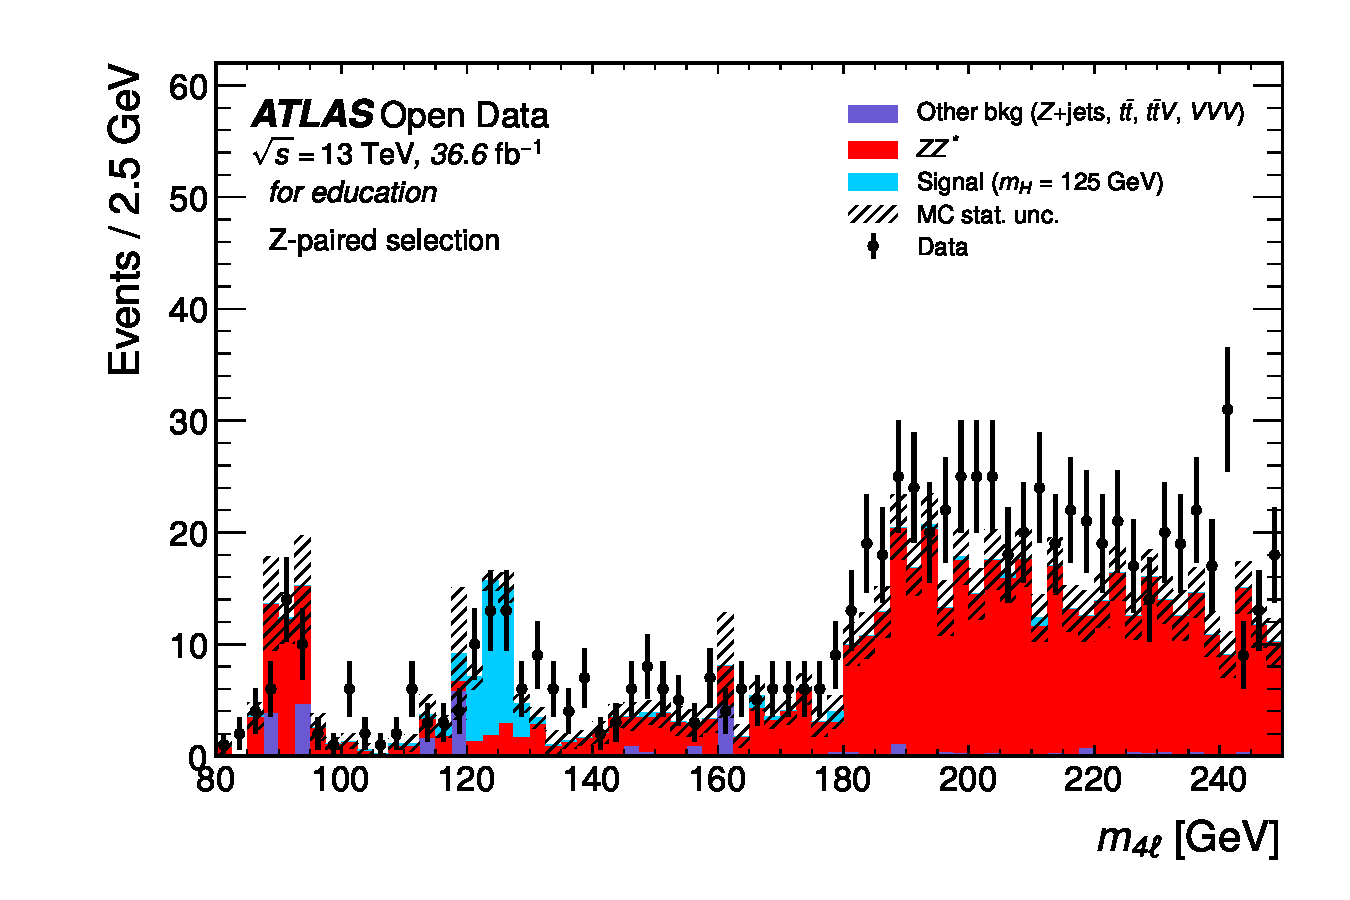
\includegraphics[width=0.72\textwidth]{m4l_paired.pdf}
\caption{$\mfl$ after the corrected selection: data and stacked simulation with its
statistical uncertainty.}
\label{fig:m4l}
\end{figure}

\section{Higgs boson mass}

\paragraph{Model.} The $N=84$ data events in $110<\mfl<140\GeV$ are fitted with the extended
unbinned likelihood
\begin{equation}
-\ln L(m_H, N_s, N_b) = N_s + N_b - \sum_{i=1}^{N}
\ln\!\left[N_s\, f_s(m_i;\, m_H+\delta) + N_b\, f_b(m_i)\right],
\end{equation}
minimized with MINUIT~\cite{minuit} through iminuit. The signal shape $f_s$ is a double-sided
Crystal Ball (a Gaussian core of width $\sigma = 2.08\GeV$ with power-law tails), whose width
and tail parameters are fixed from a weighted fit to the $H\to ZZ^*\to4\ell$ simulation with
even event numbers. The fitted peak sits $\delta = -0.350 \pm 0.010\GeV$ below the generated
mass, because of final-state radiation and energy loss, and this offset is subtracted through
$f_s(m; m_H + \delta)$. The background $f_b$ is an exponential with its slope fixed from the
$ZZ^*$ simulation; a second-order polynomial improved $-2\ln L$ by only 1.2 and was not used.
The uncertainty on $m_H$ is the MINOS interval, $-2\Delta\ln L = 1$ with $N_s$ and $N_b$
profiled.

\paragraph{Validation on simulation.} 2000 toy experiments at the simulated yields
($N_s = 39.1$, $N_b = 27.6$) all converge and give a pull
$(\hat m_H - m_H)/\sigma_{\hat m_H}$ with mean $-0.010 \pm 0.023$ and width
$1.013 \pm 0.016$: the uncertainty is correctly calibrated. The median expected uncertainty
is $0.50\GeV$. The odd-event simulation, unused for the shape and the calibration, fitted as
weighted pseudo-data, returns $m_H = 125.15 \pm 0.44\GeV$ for a generated $125.0\GeV$.

\paragraph{Result.} The fit to data (Figure~\ref{fig:massfit}) gives
\begin{equation}
m_H = 125.06^{+0.93}_{-0.92}\GeV \quad\text{(statistical only)},
\end{equation}
with a Poisson deviance of 5.9 for 9 degrees of freedom ($p = 0.75$). It agrees with the
ATLAS four-lepton measurement on 36.1\,fb$^{-1}$ of the same 2015--2016 data,
$124.79\pm0.37\GeV$~\cite{atlas2018mass}, and with the PDG average
$125.13\pm0.11\GeV$~\cite{pdg2026}, within a third of my uncertainty. Since the ATLAS result
uses the same collisions, the agreement with it is a consistency check, not an independent
test. My uncertainty is almost twice the expected $0.50\GeV$. Below $130\GeV$ the data agree
with simulation (16 against 16.7 events in 110--120\GeV, 42 against 42.6 in 120--130\GeV), but
130--140\GeV\ holds 26 events where 7.4 are predicted. With its shape fixed, the background
rises everywhere to follow this sideband ($N_b = 59.1\pm9.8$, $N_s = 24.9\pm7.9$), which
widens the likelihood. Only 0.9\% of the toys at simulated yields have an error this large;
at the fitted yields 30\% do. A Gaussian signal shape moves $\hat m_H$ by $+0.91\GeV$ on data
(spread $0.67\GeV$ in toys), so the shape choice matters at the level of the statistical error.

\begin{figure}[t]
\centering
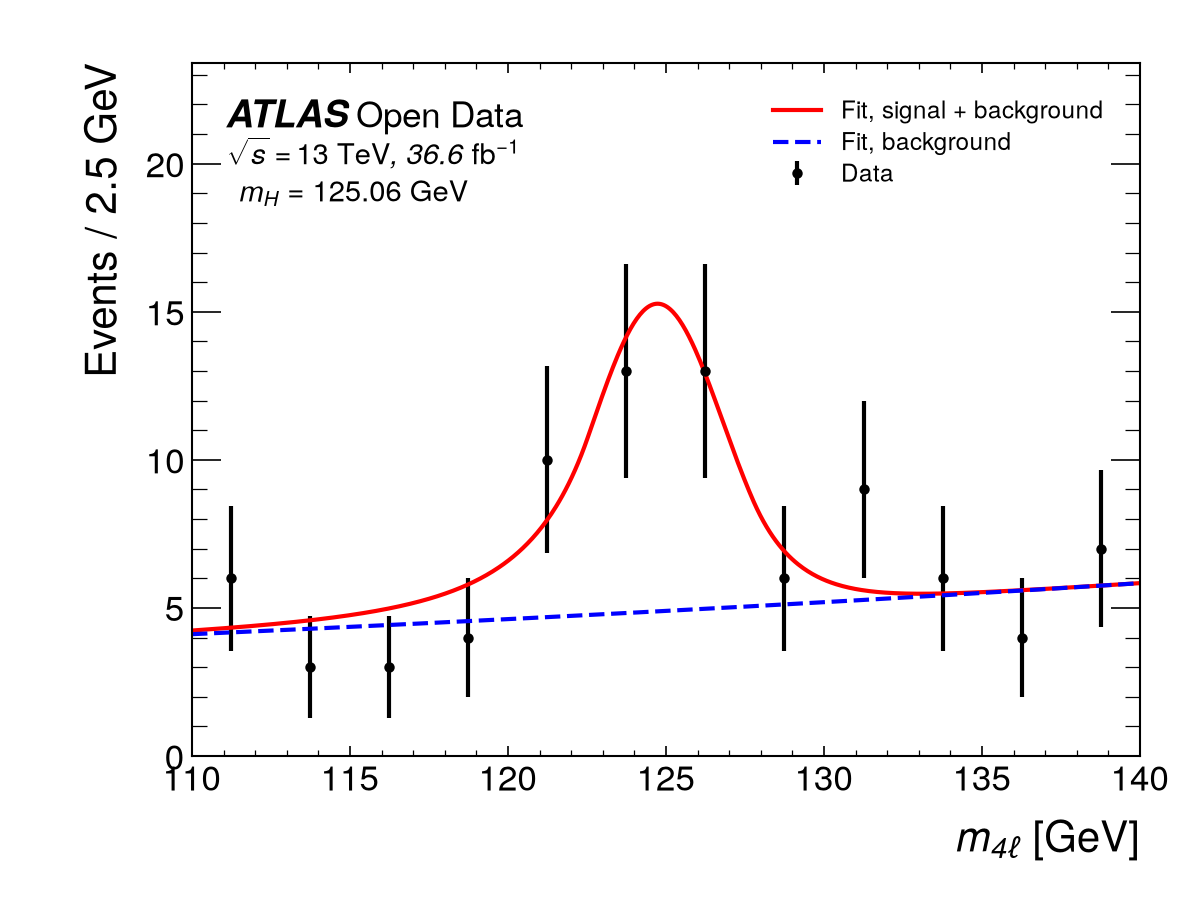
\includegraphics[width=0.49\textwidth]{mass_fit_data.png}\hfill
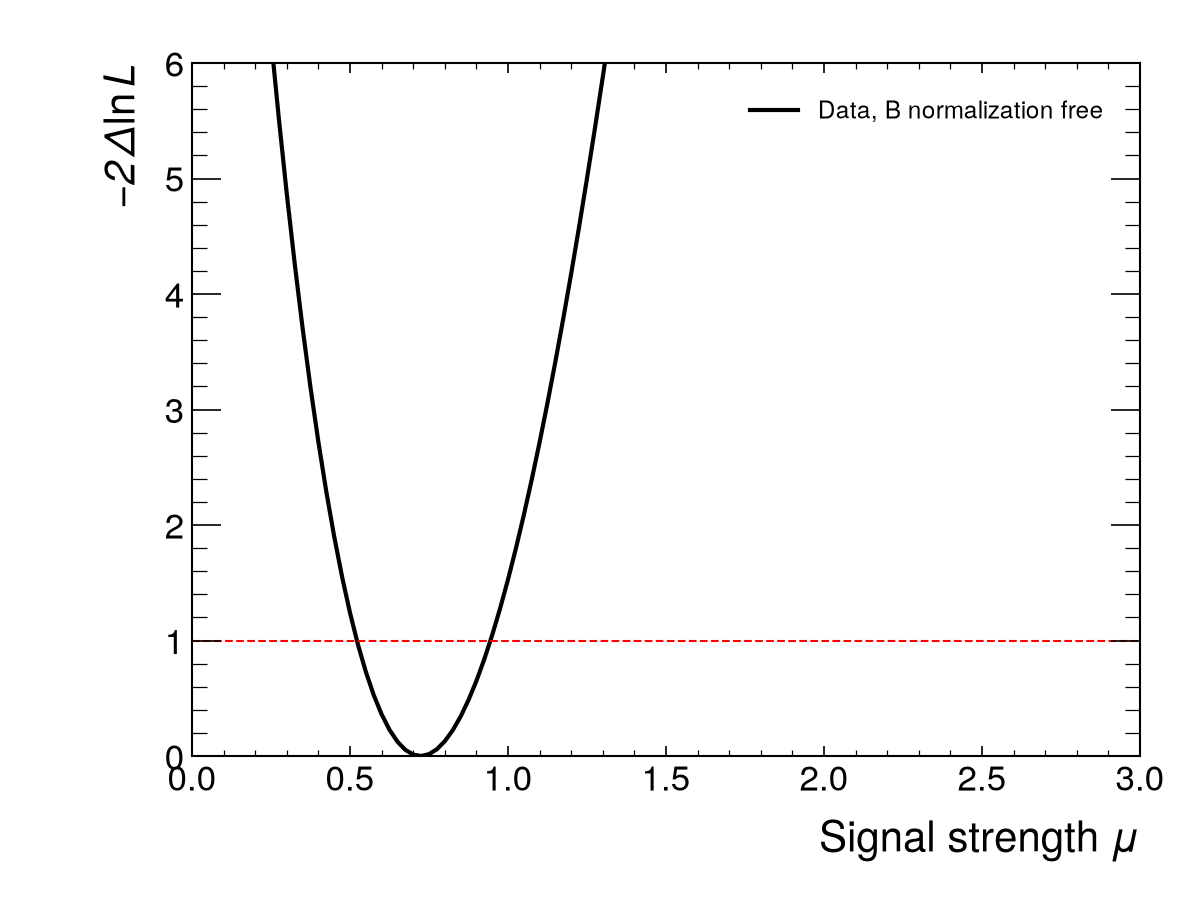
\includegraphics[width=0.49\textwidth]{significance_scan_data.png}
\caption{Left: unbinned fit of $\mfl$ in data, shown in 2.5\GeV\ bins. Right: profile
likelihood of the signal strength $\mu$ in data, with the background normalization free.}
\label{fig:massfit}
\end{figure}

\section{Significance with a profile likelihood}
\label{sec:significance}

\paragraph{Model.} The $\mfl$ spectrum in 110--160\GeV\ (20 bins of 2.5\GeV, 124 data events)
is modelled with pyhf~\cite{pyhf}, in the HistFactory form: in each bin
$\nu_i = \mu\,\kappa_L\,\gamma_i\, s_i + \mu_b\,\gamma_i\, b_i$, with the signal strength $\mu$
as parameter of interest, a free background normalization $\mu_b$, a luminosity factor
$\kappa_L$ constrained to 0.87\%~\cite{atlaslumi}, and one factor $\gamma_i$ per bin for the
simulation's statistical uncertainty. The background normalization is free because of the
40\% deficit at high mass; this was decided before the fit to data. The test statistic is
$q_0 = -2\ln[L(\mu{=}0,\hat{\hat\theta})/L(\hat\mu,\hat\theta)]$ and $Z=\sqrt{q_0}$ in the
asymptotic approximation~\cite{cowan2011}.

\paragraph{Validation.} Single-bin pyhf models reproduce the closed-form Asimov significance,
with and without a background uncertainty, within the $10^{-3}$ relative tolerance of the
tests; the background uncertainty is a Poisson-constrained (\texttt{shapesys}) term, which is
the on/off problem behind the closed-form formula. On the full model, the median of 1000
signal-plus-background toys is $6.50\pm0.04$ against the Asimov $6.64$: the asymptotic
formula is slightly optimistic. For $s=10$, $b=5$, $10^7$ counting toys give
$p_0 = 2.31\times10^{-4}$ against the asymptotic $1.59\times10^{-4}$.

\paragraph{Result.} The observed significance is $Z = 3.96$ ($p_0 = 3.8\times10^{-5}$), and
$\hat\mu = 0.72^{+0.22}_{-0.20}$ (Figure~\ref{fig:massfit}, right). The expected significance
is 6.64. The gap has two parts: the fitted background is 1.8 times the simulated one (96.6
against 53.7 events), which by itself lowers the expected value to 5.18, and $\hat\mu$ is
$1.3\sigma$ below 1. Both agree with the mass fit. Table~\ref{tab:z} shows how much the
common shortcuts overstate the significance.

\begin{table}[t]
\centering
\small
\begin{tabular}{lccc}
\toprule
Method & Notebook & Expected & Observed \\
\midrule
Notebook metric $(S{+}B)/\sqrt{B+0.3B^2}$, window & 4.43 & 7.96 & -- \\
$S/\sqrt{B}$, window & 5.74 & 11.19 & -- \\
Counting Asimov, known $B$, window & 4.70 & 7.82 & -- \\
Counting Asimov, 30\% $B$ uncertainty, window & 3.08 & 5.38 & -- \\
Shape fit, $B$ fixed to simulation & -- & 8.74 & not valid \\
\textbf{Shape fit, $B$ normalization free} & -- & 6.64 & \textbf{3.96} \\
Same, 5\GeV\ bins & -- & 6.37 & 4.18 \\
\bottomrule
\end{tabular}
\caption{Discovery significance by method. ``Window'' is $122.5<\mfl<130\GeV$; shape fits use
110--160\GeV. Expected and observed use the corrected selection. The notebook column also differs by abs weights and 7 instead of 8 signal
samples. The fixed-background fit to data is not valid: the data reject that normalization.}
\label{tab:z}
\end{table}

\section{Classifier}

\paragraph{Method.} The classifier separates signal from all backgrounds with ten features:
the four lepton $p_T$, $m_{12}$, $m_{34}$, the $p_T$ and rapidity of the four-lepton system,
$\cos\theta^*$ of $Z_1$ in the four-lepton rest frame, and the smallest $\Delta R$ between
leptons. $\mfl$ is not a feature, so that the spectrum stays usable for the fit. It is trained
on simulation with even event numbers, using absolute weights (negative weights cannot be
used as training weights), and evaluated on odd event numbers with signed weights and yields
doubled. A score threshold, chosen on the training half, defines two categories, which are
fitted together with the model of Section~\ref{sec:significance}, each with its own free
background normalization.

\paragraph{A model change, on simulation.} The planned gradient-boosted
trees~\cite{sklearn} overtrained: only 289 background events are available for training,
and the train and test background scores disagreed (Kolmogorov--Smirnov $p = 8.6\times
10^{-14}$, even with small trees). Following a rule fixed before that test, the analysis
switched to logistic regression on the same features, which shows no overtraining (KS
$p = 0.98$ for signal, 0.43 for background).

\paragraph{Result.} The ROC AUC is 0.702 on the test half. The high-score category is purer
($S/B = 2.2$ against 0.7), but the expected significance on the test half is 5.97 with two
categories against 6.06 inclusive: no gain. The purer category holds only about five
background events, whose free normalization must be fixed by its own sidebands, and the
threshold chosen on the training scores is tighter than the test half supports. Although
$\mfl$ is not a feature, the score partly learns it: the background in the high category sits
9\GeV\ lower in $\mfl$, which a $\chi^2$ shape test with so few events does not detect
($p = 0.37$). On data, with the classifier and threshold frozen, the two-category fit gives
$Z = 3.29$ against 3.90 inclusive with the same templates. The inclusive result of
Section~\ref{sec:significance} remains the main one.

\section{Limitations}

\begin{itemize}\itemsep0pt
\item The data exceed the simulation by 40\% at high mass and by a factor 3.5 at
130--140\GeV; neither cause is identified. The free background normalization absorbs the
first, but the background shape is taken from simulation.
\item Few systematic uncertainties: luminosity, a free background normalization and the
simulation's statistical uncertainty in the significance; none on the mass (no lepton energy
or momentum scale variations). The signal-shape choice alone moves $m_H$ by up to 0.9\GeV.
\item The background simulation is sparse: one $Z$+jets event of weight 5.8 is 11\% of the
background in 110--160\GeV, and 289 background events are all the classifier can learn from.
\item The selection is simplified: no $\mfl$-dependent $m_{34}$ cut, no $\Delta R$ cut, no
$J/\psi$ veto. The mass calibration comes from a single simulated mass point.
\item Blinding is partial: the data were plotted at the selection stage; every later choice
was fixed on simulation before the corresponding fit to data.
\end{itemize}

\section{Conclusion}

With 36.6\,fb$^{-1}$ of open 13\,TeV data, the four-lepton channel gives
$m_H = 125.06^{+0.93}_{-0.92}\GeV$ and an observed significance of $3.96\sigma$, with methods
that were validated on simulation and toys before being applied to data. The main lesson is
that honest statistics change the answer: in the corrected selection, a naive $S/\sqrt{B}$ of
11.2 becomes an expected 6.64 and an observed 3.96 once the background normalization is
constrained by the data instead of assumed. Better
background simulation, not a better classifier, is what this analysis needs most.

\begin{thebibliography}{9}\small\itemsep0pt
\bibitem{atlas2012} ATLAS Collaboration, Observation of a new particle in the search for the
Standard Model Higgs boson with the ATLAS detector at the LHC, Phys.\ Lett.\ B 716 (2012) 1,
arXiv:1207.7214.
\bibitem{cms2012} CMS Collaboration, Observation of a new boson at a mass of 125\,GeV with
the CMS experiment at the LHC, Phys.\ Lett.\ B 716 (2012) 30, arXiv:1207.7235.
\bibitem{opendata} ATLAS Collaboration, ROOT ntuple format 2015--2016 proton-proton Open Data
for Education and Outreach beta release from the ATLAS experiment, CERN Open Data Portal
(2025), doi:10.7483/OPENDATA.ATLAS.B5M9.44TN.
\bibitem{notebook} ATLAS Open Data, \texttt{HZZAnalysis.ipynb}, \url{https://github.com/atlas-outreach-data-tools/notebooks-collection-opendata}, directory
\texttt{13-TeV-examples/uproot\_python}.
\bibitem{cowan2011} G.~Cowan, K.~Cranmer, E.~Gross, O.~Vitells, Asymptotic formulae for
likelihood-based tests of new physics, Eur.\ Phys.\ J.\ C 71 (2011) 1554, arXiv:1007.1727.
\bibitem{minuit} F.~James, M.~Roos, Minuit: a system for function minimization and analysis
of the parameter errors and correlations, Comput.\ Phys.\ Commun.\ 10 (1975) 343.
\bibitem{atlas2018mass} ATLAS Collaboration, Measurement of the Higgs boson mass in the
$H\to ZZ^*\to4\ell$ and $H\to\gamma\gamma$ channels with $\sqrt{s}=13$\,TeV $pp$ collisions
using the ATLAS detector, Phys.\ Lett.\ B 784 (2018) 345, arXiv:1806.00242.
\bibitem{pdg2026} F.~Takahashi et al.\ (Particle Data Group), Review of Particle Physics,
Int.\ J.\ Mod.\ Phys.\ A 41 (2026) 2630011.
\bibitem{pyhf} L.~Heinrich, M.~Feickert, G.~Stark, K.~Cranmer, pyhf: pure-Python
implementation of HistFactory statistical models, J.\ Open Source Softw.\ 6 (2021) 2823.
\bibitem{atlaslumi} ATLAS Collaboration, Luminosity determination in $pp$ collisions at
$\sqrt{s}=13$\,TeV using the ATLAS detector at the LHC, Eur.\ Phys.\ J.\ C 83 (2023) 982,
arXiv:2212.09379.
\bibitem{sklearn} F.~Pedregosa et al., Scikit-learn: machine learning in Python, J.\ Mach.\
Learn.\ Res.\ 12 (2011) 2825.
\end{thebibliography}

\end{document}
